\section{Теоретические сведения}

Под \textit{нониусом} понимают дополнение к обычному масштабу прибора, позволяющее повысить точность измерения в $10\div20$ раз. Таким приспособлением снабжены штангенциркуль --- прибор для измерения длин, --- а так же буссоль и кипрегель --- приборы для измерения углов.

\begin{figure}[h]
	\begin{center}
		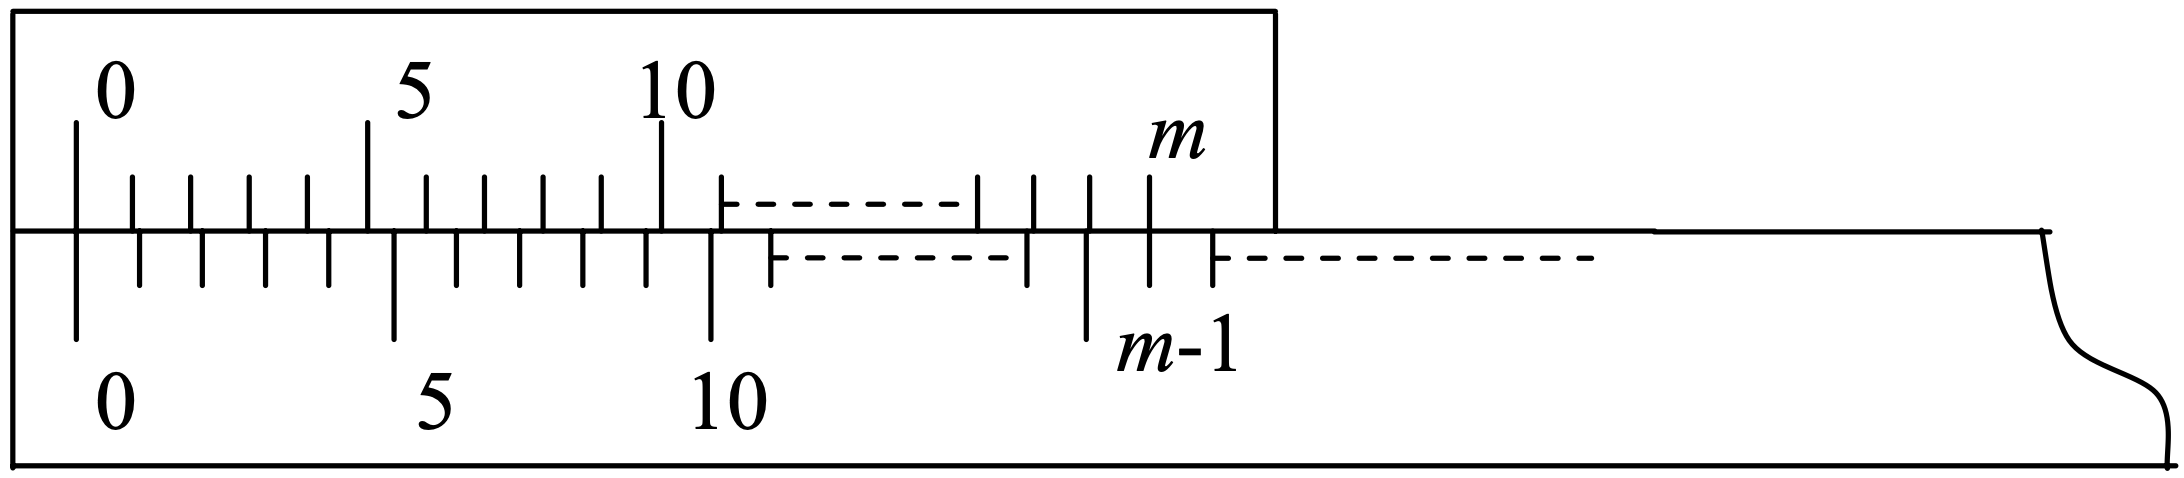
\includegraphics[width=0.7\textwidth]{pictures/PictureOne}
		\caption{Линейный нониус}\label{PicOne}
	\end{center}
\end{figure}

На рисунке~\ref{PicOne} изображён нониус, который имеет вид меньшей из двух линеек. При этом сам нониус имеет~$m$ делений. Расстояние между нулевым и последним делением нониуса равно расстоянию между нулевым и $(m-1)$-м делением основного масштаба (основной, большей линейки). Обозначим цену деления нониуса через $x$, а через $y$ --- цену деления масштаба. Тогда, из сказанного выше очевидно, что
\[
mx=(m-1)y\Rightarrow x=y- \frac{y}{m}.
\]
Точность нониуса определяется, как
\[
\Delta x=y-x=\frac{y}{m}.
\]

При измерении длины $L$ отрезка необходимо совместить ноль основного масштаба с его началом, а ноль нониуса --- с концом. Конец отрезка окажется между $k$-м и $(k+1)$-м делениями основной линейки. При этом на нониусе найдётся деление $n$, ближе всего подходящее делению $k+n$ масштаба (рис.~\ref{PicTwo}).

\begin{figure}[h]
	\begin{center}
		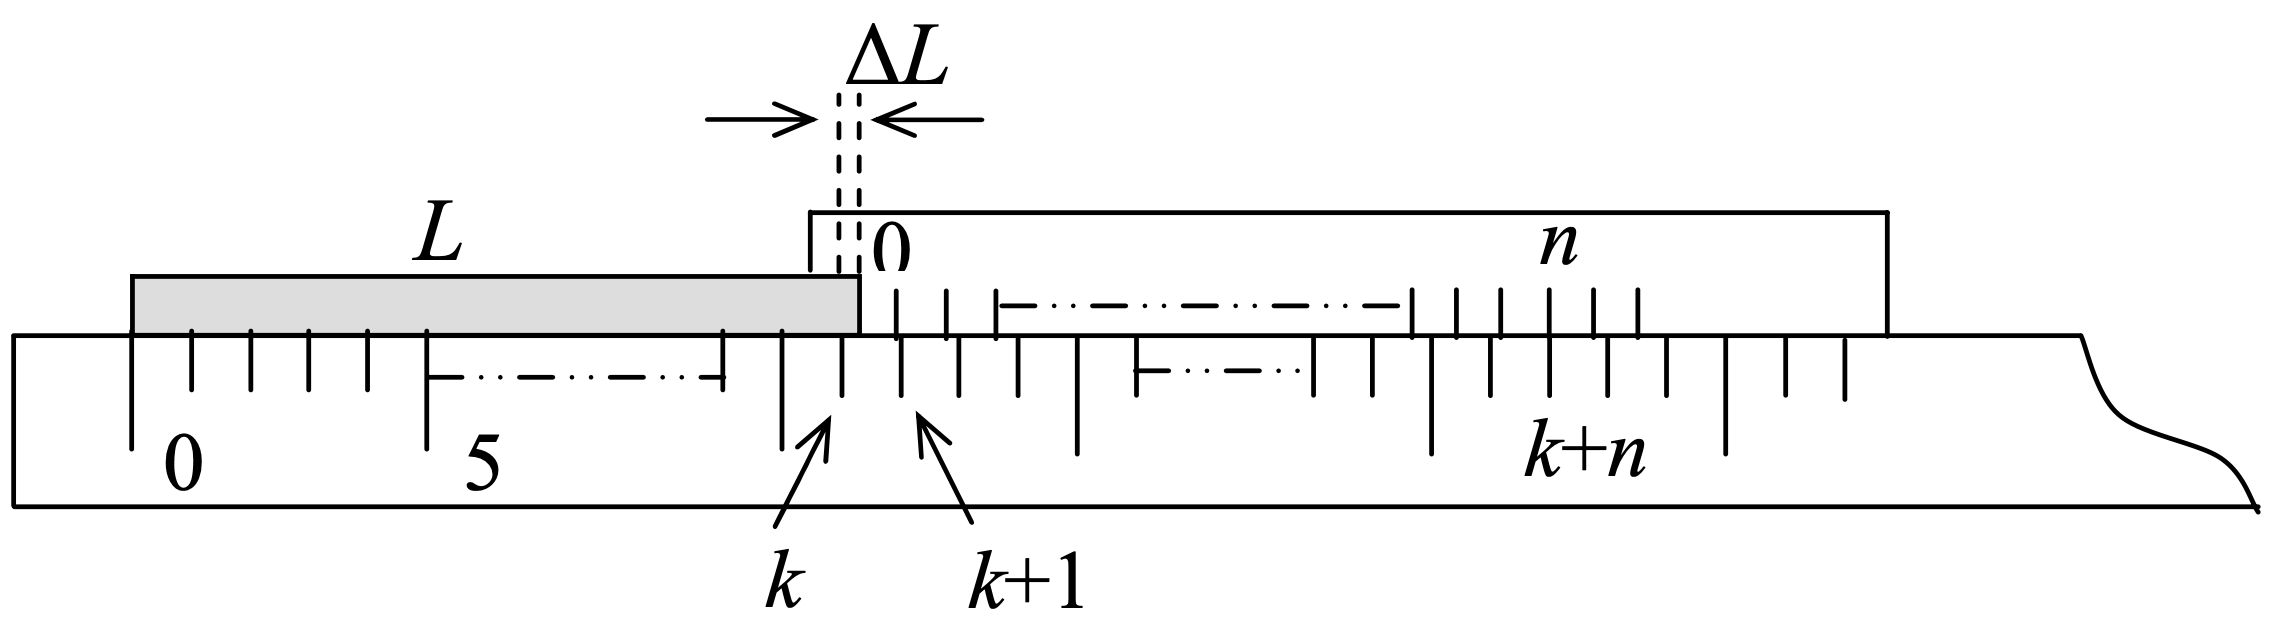
\includegraphics[width=0.7\textwidth]{pictures/PictureTwo}
		\caption{Линейный нониус}\label{PicTwo}
	\end{center}
\end{figure}

Как видно из рисунка, длина интересующего нас отрезка равна $L$. Тогда
\[
L=ky+\Delta L,
\]
где
\[
\Delta L=ny-nx=n(y-x)=n\,\Delta x.
\]
То есть
\[
L=ky+n\,\Delta x.
\]

Абсолютная погрешность нониуса равна, очевидно, половине его точности:
\[
\Delta l_\text{пр}=\frac{\Delta x}{2}.
\]

\textit{Микрометрический винт} --- это винт с малым и достаточно точно выдержанным шагом для точных измерений размеров тел. Такие винты являются составными частями микрометров. Шаг микрометрического винта составляет $0{,}5\;\text{мм}$. Поскольку барабаная шкала микрометра содержит 50 делений, поворот на одно такое деление смещает стержень на $0{,}01\;\text{мм}$.

При измерении длины микрометром, интересующее тело помещают между стержнем и упором (см. схему микрометра далее). Вращением винта за головку доводят стержень до соприкосновения с предметом. При этом вращение останавливают при появлении характерного треска. Число целых миллиметров снимают по основной шкале, деления которой сдвинуты друг относительно друга на $0{,}5\;\text{мм}$, а десятые и сотые доли миллиметра снимают по шкале барабана.